\section{Svolgimento delle misure}
Come prima cosa è stata effettuata la calibrazione dell'apparato 
strumentale.
\begin{itemize}
	\item Si sono allineati raggio laser, reticolo di diffrazione e schermo: attraverso le viti di regolazione dello specchio abbiamo fatto incidere il raggio in maniera radente sulla scala del calibro, questo è necessario per osservare sullo schermo un numero significativo di spot luminosi, essendo $\lambda \ll d$.
	\item Si è proceduto a determinare il punto \textbf{zero}: la proiezione dell'asse della scala del calibro sullo schermo. Rispetto a questo punto sono state misurate le distanze delle frange di interferenza e la distanza $D$ dello schermo dal reticolo. Per determinare la posizione di questo punto si è preso il punto medio tra lo spot luminoso del fascio diretto del laser (ben visibile senza calibro) e quello del fascio riflesso sul calibro.
\end{itemize}
La relazione che lega le grandezze in gioco è:
$$ sin (\theta_m) =-\frac{\lambda}{d}m+sin (\theta_i)$$
Dove $m$ indica il numero della frangia di diffrazione, $d$ è il passo reticolare, $\theta_i$ e $\theta_m$ sono rispettivamente l'angolo di incidenza e l'angolo della frangia $m$-esima, $D$ è la distanza dello schermo dal reticolo.

Si è proceduto alla misura della distanza $D$ tra il punto \textbf{zero} prima determinato e il reticolo di diffrazione, la dimensione del fascio laser che incide radente sulla scala del calibro non è trascurabile, ha infatti un'estensione di $\sim \unit{10}{\centi\meter}$, bisogna tenerne conto nella stima dell'incertezza. Il risultato della misura è $D = \unit{209 \pm 3}{\centi\meter}$. Per altre considerazioni su questa misura si rimanda alla sezione 3.

Conoscendo $D$ e dalla misura delle distanze delle frange di diffrazione dal punto zero è possibile determinare i $\theta_m$ e procedere ad un fit lineare di $sin(\theta_m)$ in funzione di $m$ con coefficiente angolare $-\lambda/d$ e intercetta pari a $sin(\theta_i$.)

Le misure effettuate sono riportate in \tablename{ \ref{data}}, in appendice. Il fit eseguito fornisce i seguenti risulati:
\begin{figure}[H]
	\begin{minipage}{0.25\textwidth}
		\begin{tabular}{l}
			$\lambda/d = \unit{63.34 \pm 0.07}{\micro\meter}$ \\
			$\theta_i = (89.56 \pm 0.03) ^\circ $\\
			$corr(\lambda/d,\theta) = -0.77$\\
			$\chi^2 /\text{ndof} = 18.9 / 17 $\\
			$p_{val} = 0.33$
		\end{tabular}
	\end{minipage}
	\begin{minipage}{0.8\textwidth}
		\centering
		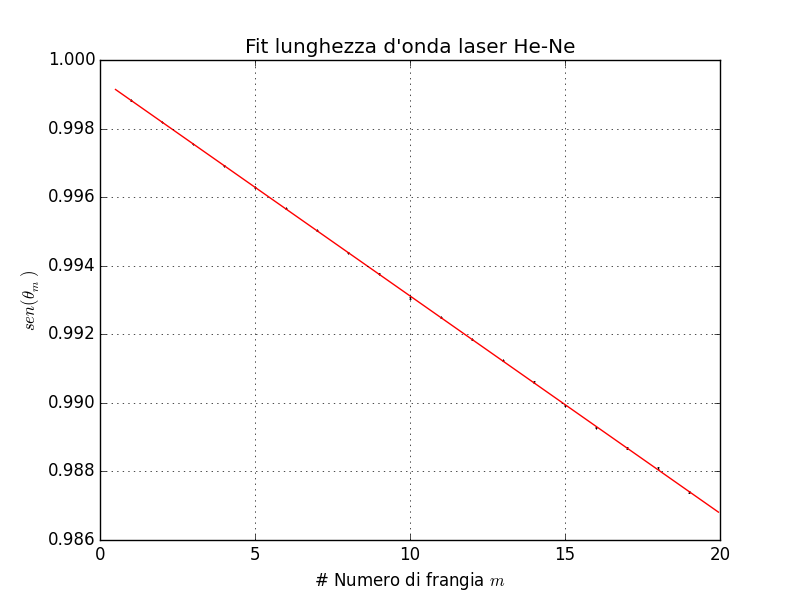
\includegraphics[width=\textwidth]{./pictures/fit_He-ne.png}
	\end{minipage}
\end{figure}

Posto un passo reticolare di $\unit{1}{\milli\meter}$, segue $\lambda = \unit{633.4 \pm 0.7}{\nano\meter}$, che è compatibile entro $1 \sigma$ con il valore riportato di $\unit{632.8}{\nano\meter}$.